\chapter{Grundstruktur der App}
\label{cha:basicstructure}
%
\begin{figure}[htp]
	\centering
	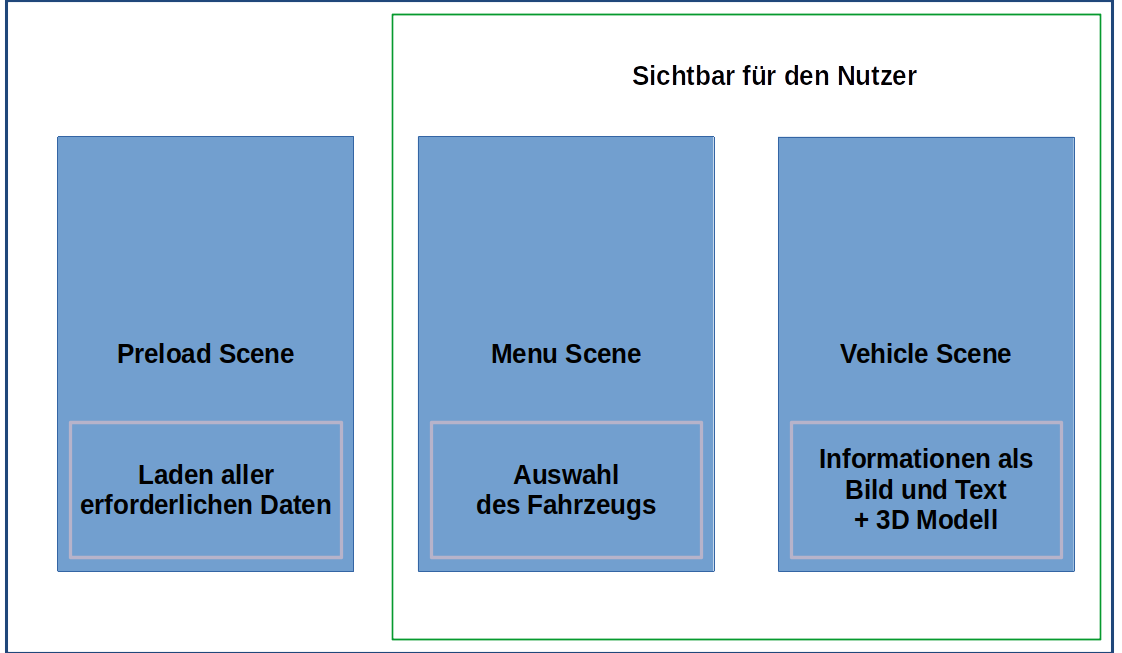
\includegraphics[width=.8\linewidth]{img/basic_structure}
	\caption[structure]{Grundstruktur und Szenenaufteilung der VMD Vorfahrt App}
	\label{fig:basicstructure}
\end{figure}

\begin{itemize}
	\item \pres
	\begin{itemize}
		\item alle erforderlichen Daten werden hier beim Start geladen
		\item Entscheidung, welche Seite angezeigt werden soll
		\item Lädt Bilder und Texte der gewählten Seite aus dem \sad
		\item 3D-Modelle sind im Build der App hinterlegt, nicht von außen änderbar
	\end{itemize}
	\item \mms
	\begin{itemize}
		\item Auswahl aller geladenen Fahrzeuge
		\item Menüeinträge werden dynamisch beim Start aus Prefab erstellt
		\item jedes Titelbild ist ein Button mit Weiterleitung zur \vhs
	\end{itemize}
	\item \vhs
	\begin{itemize}
		\item inhaltlich Umfangreichste Szene
		\item zeigt alle vorab geladenen Text- und Bildinformationen an
		\item ermöglicht Rotation des 3D-Models entlang der vertikalen Achse
		\item Alle Ansichten lassen sich in eine Vollbildansicht skalieren
	\end{itemize}
\end{itemize}
%